\documentclass[10pt,CJKmath]{ctexart}
\usepackage{MyNote}




% 定义重点高亮和公式框样式
\usepackage{framed,longtable,booktabs,array,calc}

\usepackage{etoolbox}

\AtBeginEnvironment{longtable}{\footnotesize}
\AtEndEnvironment{longtable}{\normalsize}


%参考tcolorbox P21
\NewTotalTCBox{\commandbox}{ s v }
{verbatim,colupper=white,colback=black!50!white,colframe=black,sharp corners,boxrule=0pt,left=0mm,right=0mm,top=0mm,bottom=0mm}
{\IfBooleanT{#1}{\textcolor{red}{\ttfamily\bfseries > }}%
	\lstinline[language=c++,basicstyle=\ttfamily\small,keywordstyle=\color{blue!35!white}\bfseries]^#2^}


\begin{document}

\pagestyle{fancynotes}


\part{内切球}

\section{内切球基础}
\begin{table}[H]
	\begin{longtable}{p{0.3\textwidth}p{0.3\textwidth}p{0.3\linewidth}}
		\large\textbf{锥体}&\large\textbf{柱体}&\large\textbf{台体}\\\toprule
		\kk{1}\textbf{三棱锥}\newline\kk{2}\textbf{正棱锥}\newline\kk{3}\textbf{圆锥}&\kk{1}\textbf{正方体}\newline\kk{2}\textcolor{red}{直柱体}\newline\kk{3}\textcolor{red}{圆柱}&\kk{1}\textcolor{red}{正台体}\newline\kk{2}\textcolor{red}{圆台}\\
	\end{longtable}
	\caption{常见几何体内切球：黑体一定存在内切球，\textcolor{red}{红}色字体\emph{可能有}内切球}
\end{table}
对于可能有的解释：可能有表示有前提。例如对于直棱柱，如果题目说有内切球，这就是前置条件。
\subsection{一定有内切球的如何找到球心及半径}
\begin{enumerate}
	\item \textbf{三棱锥：}对于普通棱锥有相对来说的万能公式：\colorbox{blue!10}{$r=\dfrac{3V}{S}$}。
	
	证明过程\textbf{类似三角形内切圆}：对于任意$\triangle ABC$，内切圆的半径为$r$，则有
	\[
		S=\dfrac{1}{2}ar+\dfrac{1}{2}br+\dfrac{1}{2}cr=\dfrac{1}{2}\big(a+b+c\big)r
	\]
	即：\colorbox{yellow}{$r=\dfrac{2 S}{a+b+c}$}，$a+b+c$是周长。
	
	在此基础之上考虑三棱锥：\\
	\begin{minipage}[c]{0.5\textwidth}
		%\centering
		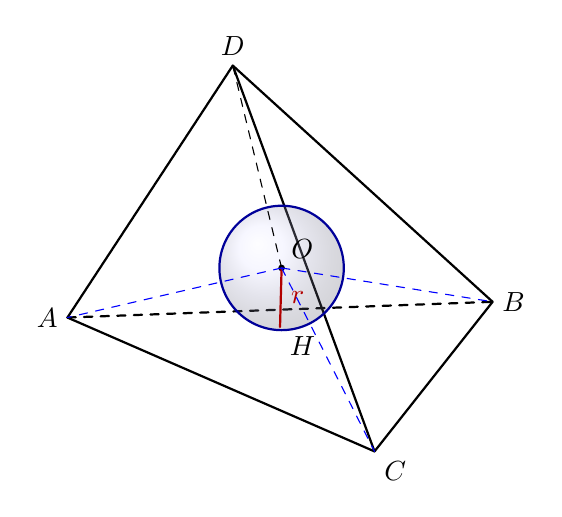
\begin{tikzpicture}[scale=1,line join=round,line cap=round,>=stealth]
			% 非标准三棱锥的四个顶点
			\coordinate (A) at (-2.8,0);
			\coordinate (B) at (2.6,0.2);
			\coordinate (C) at (1.1,-1.7);
			\coordinate (D) at (-0.7,3.2);

			% 球心与半径示意
			\coordinate (O) at (-0.08,0.63);
			\coordinate (H) at (-0.1,-0.12);
			\def\r{0.79}

			% 底面
			\draw[thick] (A) -- (C) -- (B);
			\draw[thick,dashed] (A) -- (B);

			% 侧棱
			\draw[thick] (D) -- (A);
			\draw[thick] (D) -- (B);
			\draw[thick] (D) -- (C);

			% 内切球示意
			\shade[ball color=blue!18,opacity=0.25] (O) circle (\r);
			\draw[blue!60!black,thick] (O) circle (\r);

			% 球心与半径
			\fill (O) circle (1.2pt);
			\draw[red!70!black,thick] (O) -- (H) node[midway,right] {$r$};
			\draw[dashed] (O) -- (D);

			% 绘制多个三棱锥
			\draw[dashed,blue](O)--(A);
			\draw[dashed,blue](O)--(B);
			\draw[dashed,blue](O)--(C);
			% 顶点与关键点标注
			\node[left] at (A) {$A$};
			\node[right] at (B) {$B$};
			\node[below right] at (C) {$C$};
			\node[above] at (D) {$D$};
			\node[above right] at (O) {$O$};
			\node[below right] at (H) {$H$};
		\end{tikzpicture}
	\end{minipage}
	\begin{minipage}[b]{0.45\textwidth}
	从球心O到各个顶点连线，把整个三棱锥分成4个小三棱锥。
	
	显然三棱锥体积$\equiv$4个小三棱锥体积之和，小三棱锥高为球半径r。
	
	因此有$V=\dfrac{1}{3}\big(S_1+S_2+S_3+S_4\big)\times r$
	
	\colorbox{yellow}{$\therefore\quad r=\dfrac{3V}{S}$}，S为表面积之和。
	\end{minipage}
\end{enumerate}
\end{document}